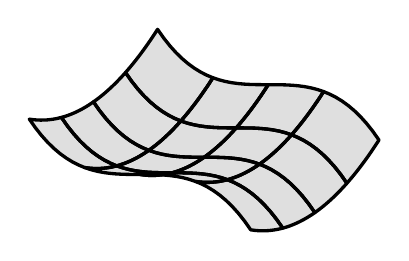
\begin{tikzpicture}[
    x=(215:2em/sqrt 2), y=(0:2em), z=(90:2em),
    declare function={f(\x,\y)=((\x-3)^2+(-\y+3)^3)/8+3;}, 
  very thick, line join=round]
%  \draw [-stealth, black!75] (0,0,0) -- (5,0,0) node [below left] {$x$};
%  \draw [-stealth, black!75] (0,0,0) -- (0,5,0) node [below right] {$y$};
%  \draw [-stealth, black!75] (0,0,0) -- (0,0,5) node [right] {$z$};

  \foreach \x in {1,...,4}
  \foreach \y in {1,...,4}{
    \draw [black, fill=black, fill opacity=0.125, 
    domain=0:1, samples=10, variable=\t] 
    plot (\x+\t, \y, {f(\x+\t,\y)}) -- 
    plot (\x+1, \y+\t, {f(\x+1,\y+\t)}) -- 
    plot (\x+1-\t, \y+1, {f(\x+1-\t,\y+1)}) --
    plot (\x, \y+1-\t, {f(\x,\y+1-\t)}) -- cycle;
  }
\end{tikzpicture}
